\section{Synthetic Images Production} \label{sec:synth_image}
    After the model is complete we have a three-dimensional representation of the tissue under study. The aim of the work is though to produce synthetic images from that structure, more precisely we want pairs of images composed of the synthetic-histological images and its related segmentation mask. The transition from 3D structure to a 2D image is the last step in the process, and it is inspired by the actual traditional technique for the preparation of the histological specimen, as described before in section \ref{ssec:samp_prep}. As the biopsy sample is treated and then sectioned with the microtome, the virtual model is sectioned in a random direction, producing an image representing the slice. This first image contains all the information of the section but its appearance is completely arbitrary and its look has nothing to share with a realistic sample. The original slice then acts perfectly as a segmentation mask, but some careful and dramatic makeover is needed to produce the final realistic looking image. In this section I will describe the general procedure to produce virtual slices from the two 3D virtual models described before in section \ref{sec:models} and the technique used to edit the images and give them the desired appearance.

\subsection{Sectioning Process} \label{ssec:sect_proc}
    For any model created following the general procedure described in \ref{sec:models}, a fortiori for the two particular models of pancreatic and dermal tissue, the sectioning process will be almost the same, and it will rely mainly on the algorithm for the general section of polyhedron described back in section \ref{ssec:pol_sec}. As stated before the models are essentially composed by labeled polyhedron spatially organized in a 3D volume. The ordered section of each polyhedron will yield all the polygons that shall be assembled in the final section.
    In Figure \ref{fig:sec_3D} is shown the three-dimensional representation of the section of a simple ramification, as the one in Figure \ref{fig:cell_id}. All the polygons that compose the section are drawn with the color correspondent to their label, following the same idea of Figure \ref{fig:cell_id}. In Figure \ref{fig:section_simple} is printed the final result of the sectioning algorithm applied to the model, which will be the segmentation mask in the single pair of synthetic images. The colors in the produced slice match the colors used for the different identities in the 3D model.

        \begin{figure}[h]
            \centering
            \begin{subfigure}[t]{0.45\textwidth}
                 \centering
                 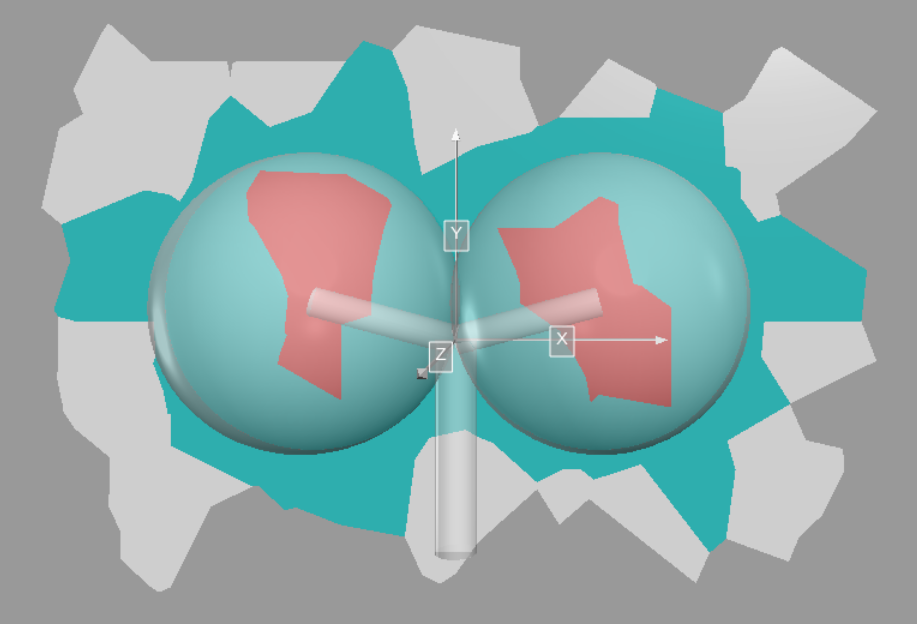
\includegraphics[width = \textwidth]{images/sec_3D}
                 \caption{2D polygonal sections represented in a 3D environment.}
                 \label{fig:sec_3D}
            \end{subfigure}
            \hfill
            \begin{subfigure}[t]{0.45\textwidth}
                 \centering
                 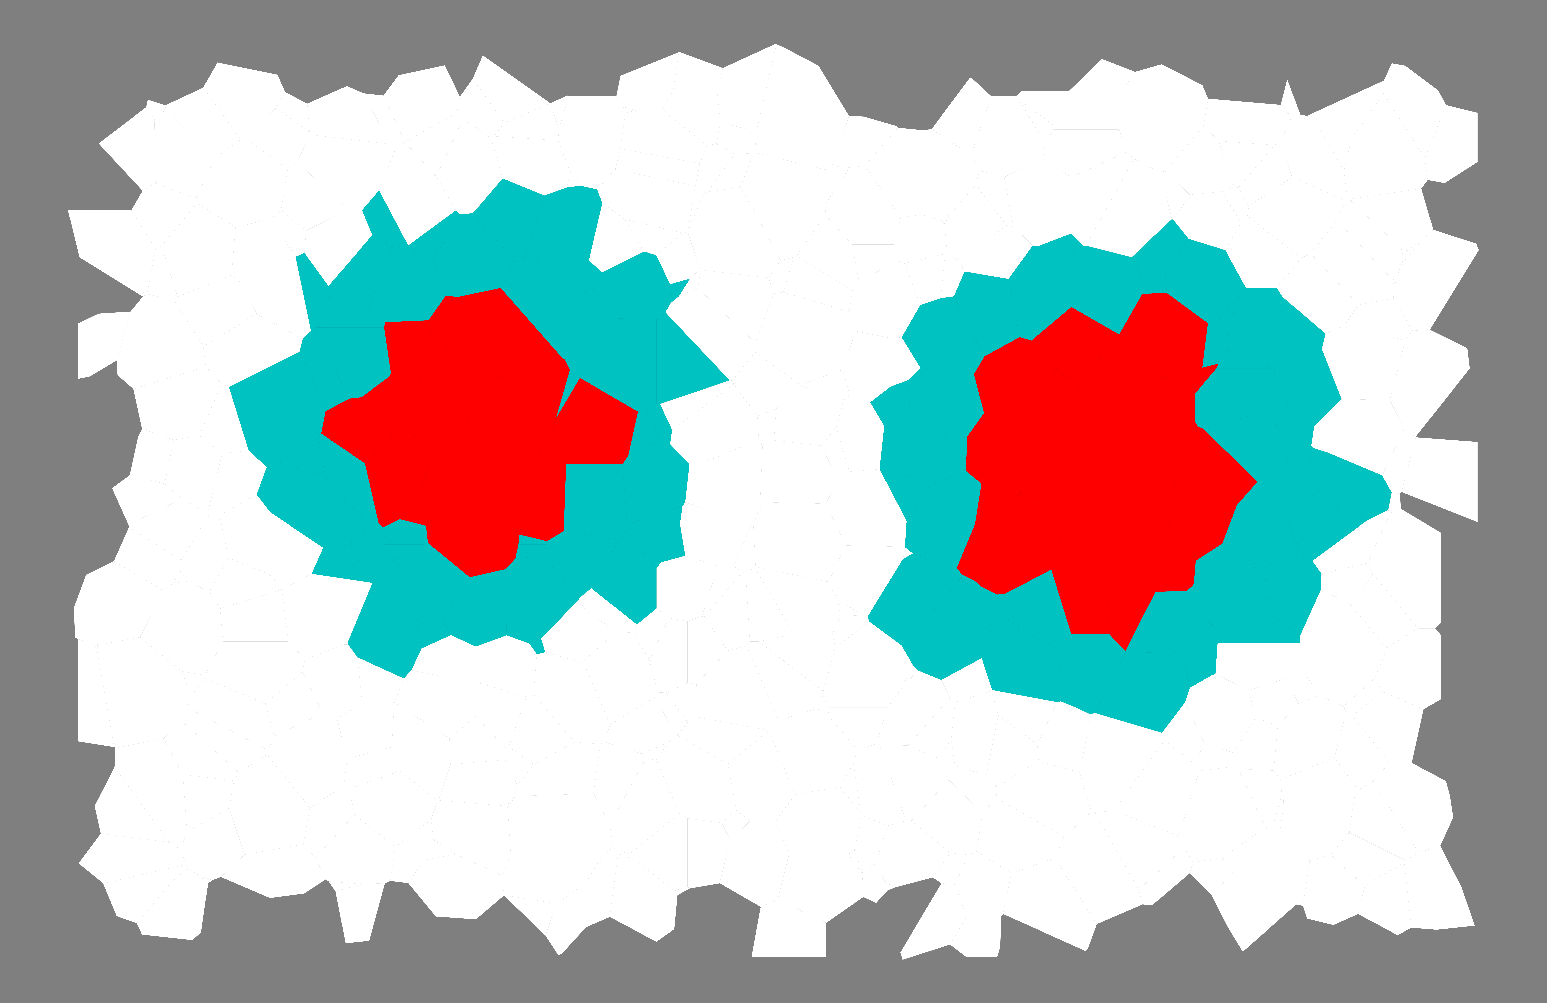
\includegraphics[width = \textwidth]{images/section_simple}
                 \caption{The fianl section image, produced directly on a planar picture, skipping completely the 3D representation.}
                 \label{fig:section_simple}
            \end{subfigure}
            \caption{In this Figure is shown the idea of the correspondence between the section of a simple structure in the space and the correspondent section. The correspondence is not perfect for representation requirments, in fact the two images even if very similar are produced with two completely different methods. At the left an image of 2D polygonal section embeded in a 3D space, made using 3D visualization tools. At the right a simple image produced printing the polygons in a planar picture. Printing 2D polygons in the space is much more complicated than one would think using the same tool used to produce the other images like Figure \ref{fig:cell_id} and \ref{fig:vor_comp}. This choice has been done for the sake of the overall homogeneity in pictures style.}
            \label{fig:first_sect}
        \end{figure}

    The simplest, yet over-abundant, way to proceed is to create the model in its entirety and subsequently choosing the sectioning plane. Afterward, it is necessary to select only the regions that intersect the plane and section them all. Actually, the test on the intersection passes through the check on the relative position of the polyhedron's vertices respect to the sectioning plane: if all the vertices lie on the same semi-space then the intersection would be null and the polyhedron is not of interest for that particular section. This procedure is exactly the first step of the algorithm in \ref{ssec:pol_sec}, thus the filtering on the regions is actually made during construction for optimization. The alternative method could be to choose in the first place the direction of the sectioning plane, and in second place to generate the model's decomposition only in the volume adjacent to that plane. This method allows enables to spare a good amount of computation, without any negative impact on the final result. The only delicate step is the choice of a wide enough region of space around the plane, which doesn't compromise the representation.

    As a guarantee for richness and diversification among the images, there is the need for some degree of controlled randomness in the sectioning process, for example in the determination of the sectioning plane direction. All the sectioning process is then based on a single starting \textit{seed}, which determines the direction of the sectioning plane in a deterministic way, and all the rest of the model is generated as a consequence. In this way, all the possible angulations are equally probable and will be sampled in view of multiple applications of this process. In Figure \ref{fig:4sph_sections} are shown two different sections, along two random planes on two simple ramified structures with four spheres.

        \begin{figure}
            \centering
            \begin{subfigure}[t]{0.2\textwidth}
                 \centering
                 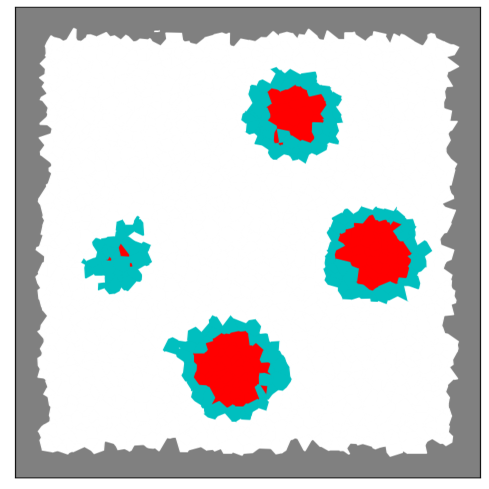
\includegraphics[width = \textwidth]{images/4sph_sec1}
                 \label{fig:4sph_sec1}
            \end{subfigure}
            \quad
            \begin{subfigure}[t]{0.2\textwidth}
                 \centering
                 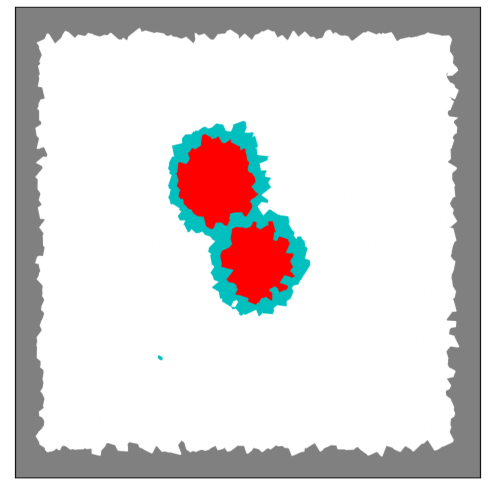
\includegraphics[width = \textwidth]{images/4sph_sec2}
                 \label{fig:4sph_sec2}
            \end{subfigure}
            \caption{Two different section, along two randon planes on two simple ramificated structure with four spheres.}
            \label{fig:4sph_sections}
        \end{figure}

\subsection{Appearance Makeover} \label{ssec:app_mkov}
    After the application of the sectioning algorithm of the previous section, the image which will act as a segmentation mask is ready. The last, and difficult task that remains is to transform the image and to give it a realistic look. I tried many different transformations, more or less complicated, and there was not a final decision on which is the best blend of them. In this section, I will describe them as an arsenal of possibilities and show their impact on the images.

    \begin{description}
        \item [Color Palette] \hfill \\
        The first correction to do to the images will inevitably be a change in the colors of the image. Gray, Turquoise, and Red are the perfect choice for label-colors but act poorly as physiological colors. In Figure \ref{fig:new_palette} is shown an example of an image produced re-mapping the colors to a new palette, inspired to the coloring of the real specimen in Figure \ref{fig:panc_struct} and [??], given by the traditional hematoxylin and eosin staining process.

        \begin{figure}[h]
            \centering
            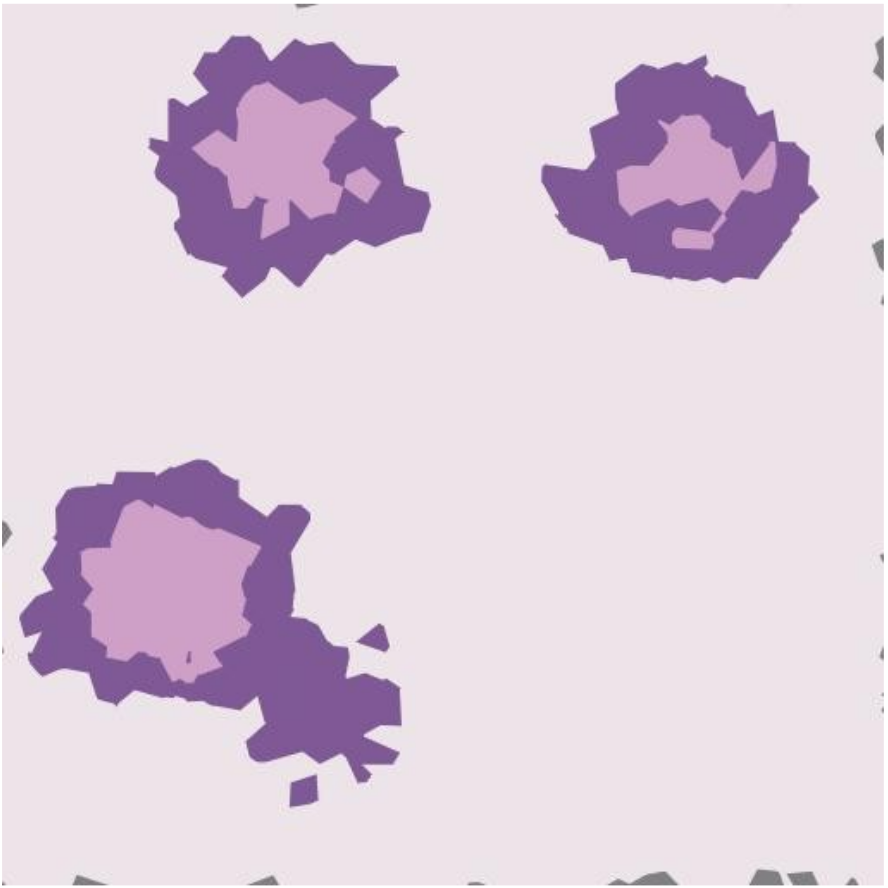
\includegraphics[width = 0.2\textwidth]{images/new_palette}
            \caption{Example of images produced re-mapping the colors with a color palette inspired to a real H\&E stained histological sample.}
            \label{fig:new_palette}
        \end{figure}

        \item [Nuclei Projection] \hfill \\
        Another fundamental processing needed was the projection of cells' nuclei on the image. Usually, nuclei are clearly visible in histological samples and guide the analysis allowing to detect individual cells in the specimen. As a reference for the nucleus position the starting point of every polyhedral region has been used and projected on the sectioning plane as a little dark purple circle. The diameter of those circles as been chosen to be a submultiple (10\%) of the linear estimated dimension $\hat{L}$ of the cells in the decomposition\footnote{Following the same logic of step 3 of section \ref{ssec:panc_tis_mod}.}.

        \begin{figure}
            \centering
            \begin{subfigure}[t]{0.2\textwidth}
                 \centering
                 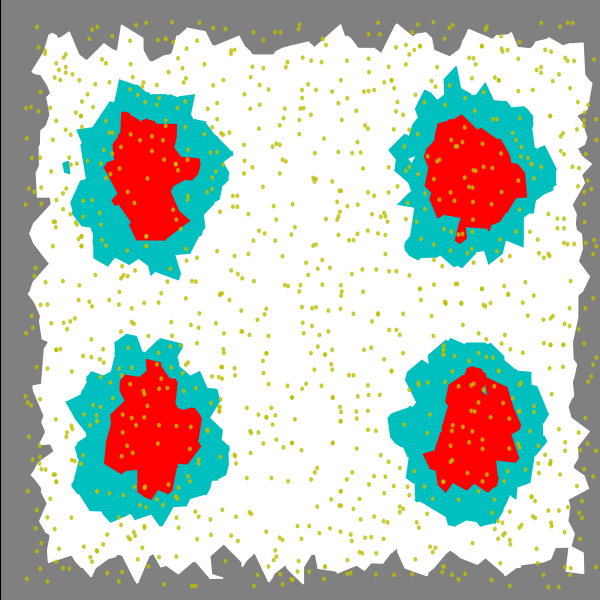
\includegraphics[width = \textwidth]{images/nuclei_mask}
                 \label{fig:nuclei_mask}
            \end{subfigure}
            \quad
            \begin{subfigure}[t]{0.2\textwidth}
                 \centering
                 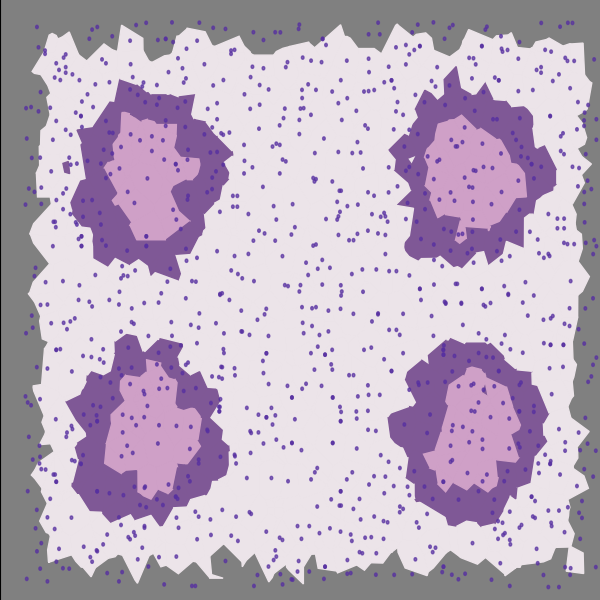
\includegraphics[width = \textwidth]{images/nuclei_real}
                 \label{fig:nuclei_real}
            \end{subfigure}
            \caption{Nuclei projection on the image: (left) in yellow in the segmentation mask and (right) in purple in the image under makeover.}
            \label{fig:nuclei_proj}
        \end{figure}

        Nuclei projection, among the other things, is an excellent tool to perceive the different effects obtained with different choices of quasi-random distributions or fully-random distributions (with reference to section \ref{ssec:saltelli}). The different impact on the overall image is huge, and it really changes the overall sense of the image. In Figure \ref{fig:sampling_comparison} are reported four different sections, produced with the same density on cells but with four different methods for the sampling of starting decomposition's points.

        \begin{figure}
            \centering
            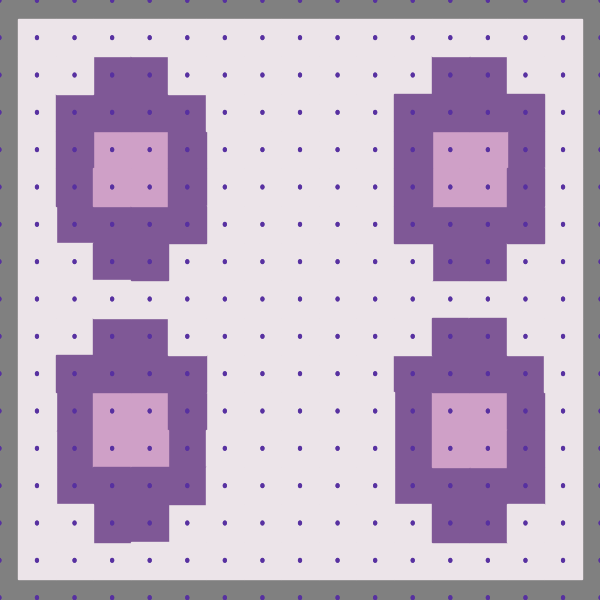
\includegraphics[width =0.24 \textwidth]{images/lattice}
            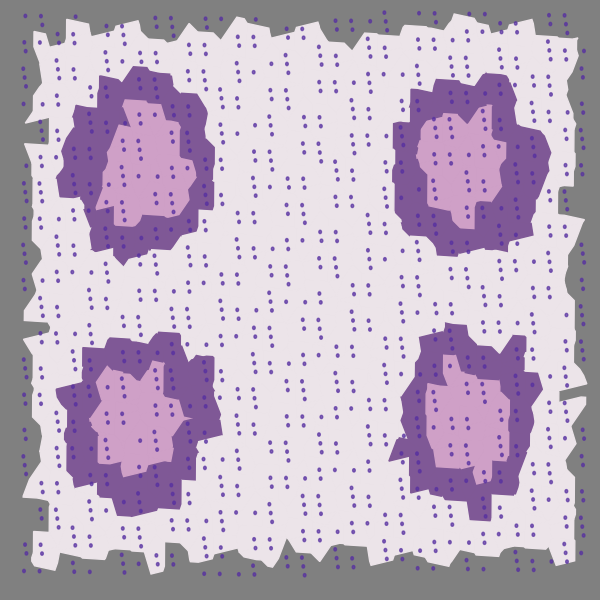
\includegraphics[width =0.24 \textwidth]{images/sequence}
            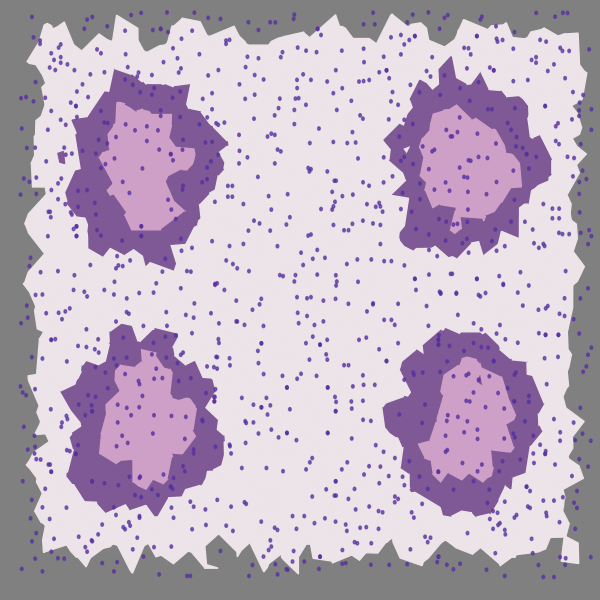
\includegraphics[width =0.24 \textwidth]{images/saltelli}
            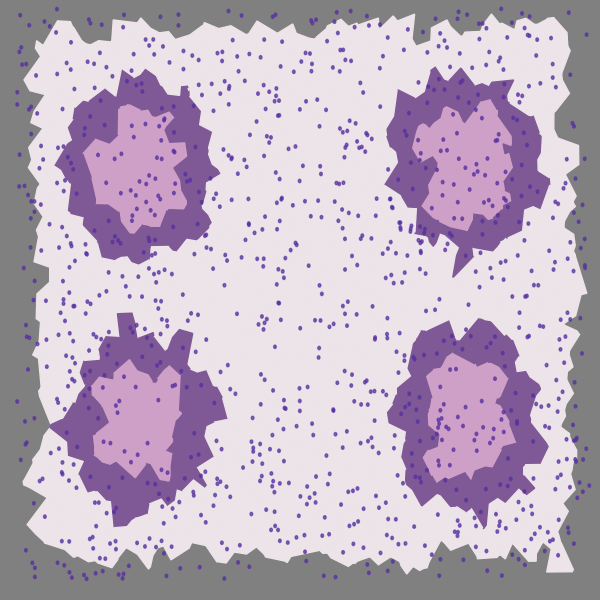
\includegraphics[width =0.24 \textwidth]{images/uniform}
            \caption{Four different sections produced with the same density on cells but with four different method for the sampling of starting decomposition's ponits (from left to right): $\bullet$ points sampled on a regular lattice, $\bullet$ sampling following a simple recursion sequence as the one in equation (\ref{eq:ad_rec}), $\bullet$ following the \textit{saltelli} algorithm, $\bullet$ following a fully-random distribution.}
            \label{fig:sampling_comparison}
        \end{figure}

        \item [Boundaries Projection] \hfill \\
        On the same wave of the previous tool, another operation which can help the appearance of an image is the projection of the boundaries of each (or just a part) of the polygonal sections. The drawing can be clearly tuned and customized depending on the specific necessities. In Figure \ref{fig:derma_slice} is shown an example of section on the dermal tissue model in \ref{ssec:derm_tis_mod}, in which the boundaries of all the cells have been lightly marked, and the boundaries of the cells in the keratine layer have been heavily marked instead.

        \begin{figure}
            \centering
            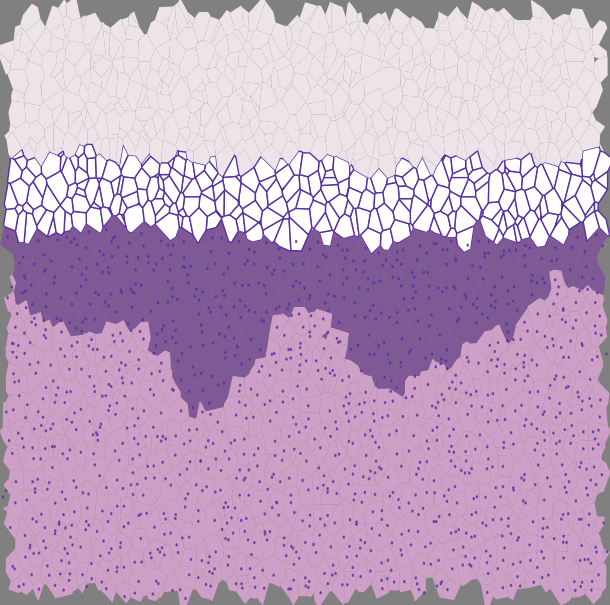
\includegraphics[width = 0.4\textwidth]{images/derma_slice}
            \caption{Example of images produced re-mapping the colors with a color palette inspired to a real H\&E stained histological sample.}
            \label{fig:derma_slice}
        \end{figure}

        \item [Blurring Effects] \hfill \\
        In all the images produced so far the boundaries between polygonal sections are perfectly sharp and without any smudge. To give a more realistic feeling to those pictures I tried different forms of blurring. As the first try, I applied a Gaussian blurring filter, which is an extremely common blurring operation in computer vision, which consists of a simple discrete convolution with a 2D Gaussian kernel. The effect is a regular and diffuse blur all over the image, as in Figure \ref{fig:gauss_blurr}. The second blurring effect I implemented was based instead on the averaging of parallel and adjacent slices on the same model. This method is inspired by the real sectioning technique, in which every slice is not an infinitesimal layer of matter, but a finite sample, which suffers from mechanical dragging during the operation. The idea is that the average between three or more slices equally spaced above and below the \textit{main} slice should recreate a realistic blurring effect. An example of an image produced with this process is shown in Figure \ref{fig:av_blur}.

        \begin{figure}
            \centering
            \begin{subfigure}[t]{0.2\textwidth}
                 \centering
                 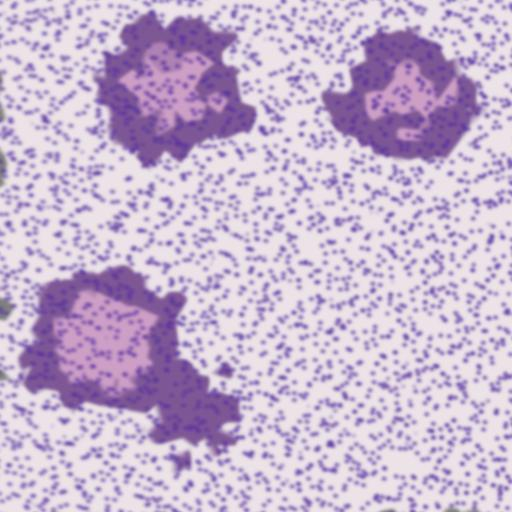
\includegraphics[width = \textwidth]{images/gauss_blurr}
                 \caption{}
                 \label{fig:gauss_blurr}
            \end{subfigure}
            \quad
            \begin{subfigure}[t]{0.2\textwidth}
                 \centering
                 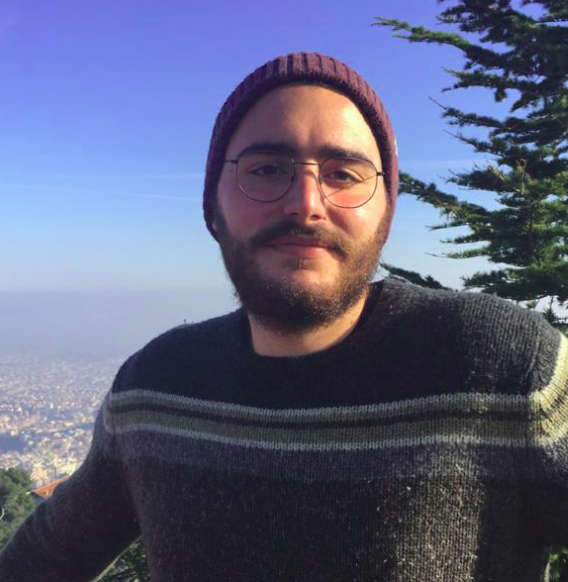
\includegraphics[width = \textwidth]{images/me}
                 \caption{}
                 \label{fig:av_blur}
            \end{subfigure}
            \quad
            \begin{subfigure}[t]{0.2\textwidth}
                 \centering
                 
\includegraphics[width = \textwidth]{images/rgb_prlin}
                 \caption{}
                 \label{fig:rgb_prlin}
            \end{subfigure}

            \caption{The two blurring effects used in this work: (left) A standard Gaussian-filter blur and (center) a specific blur introduced averaging adjacent parallel slices on the same image. (right) An example of RGB color noise built joining three different Perlin noise surfaces, one for each color channel.}
            \label{fig:blur_effect}
        \end{figure}

        \item [Perlin RGB Noise] \hfill \\
        A further attempt to give visual texture to the image was done using again the Perlin noise, described in section \ref{ssec:perlin}. The idea is to create some fluctuation among the color channels of the image around the sharp values of the image produced by the sectioning algorithm.
        From a practical point of view I created three different and independent Perlin noise surfaces, one for every color channel (Red, Green, and Blue), and added them to create a RGB noise on the image. An example of the resulting image is shown in Figure \ref{fig:rgb_prlin}.

        \item [Style Transfer] \hfill \\
        This last tool I will describe is the most sophisticated so far. It consists of the application of a style-transfer neural network (STNN) on the image obtained through the sectioning process, for the implantation of the visual texture from a real sample of the corresponding tissue. Style-transfer NNs, and their functioning, have been described in detail in section \ref{ssec:sttrNN}, and here I will cover just the particular applications on the two type of section produced.

        The first manipulation I report is the one on a section from the pancreatic tissue model. The image of which to conserve the visual content is a section with some simple pre-processing picked from the ones described before (Figure \ref{fig:st_nn1}): a more accurate color palette, the projection of nuclei, and the average on five adjacent slices. The image from which to pick the style, thus the visual texture, is a portion of an actual histological sample of pancreas, and it is shown in Figure \ref{fig:st_nn2}. The application of the STNN yields an hybrid image, shown in Figure \ref{fig:st_nn3}. The second application was made on a section on dermal tissue. The three content, style and styled images are shown respectively in Figure \ref{fig:st_nn4}, \ref{fig:st_nn5}, and \ref{fig:st_nn6}.

        \begin{figure}
            \centering
            \begin{subfigure}[t]{0.3\textwidth}
                 \centering
                 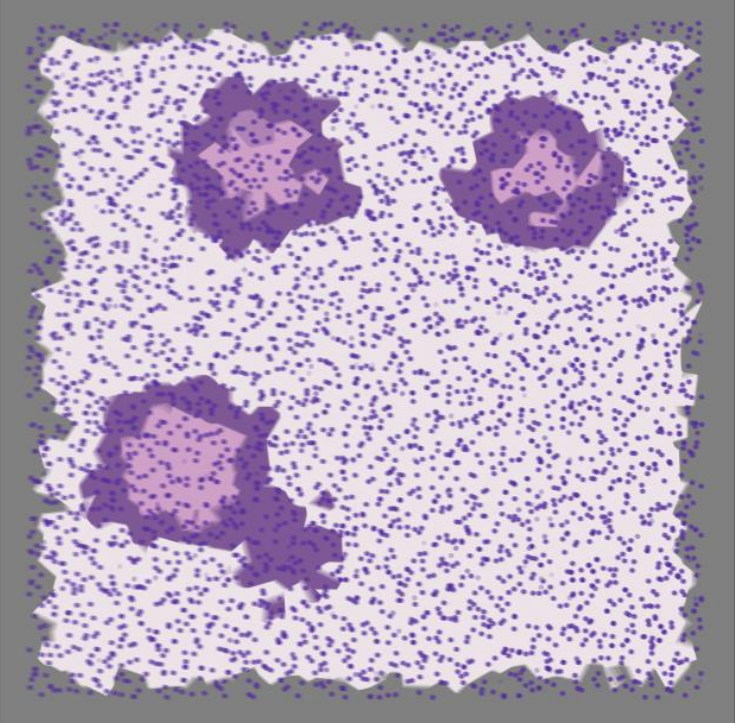
\includegraphics[width = \textwidth]{images/st_nn1}
                 \caption{}
                 \label{fig:st_nn1}
            \end{subfigure}
            \quad
            \begin{subfigure}[t]{0.3\textwidth}
                 \centering
                 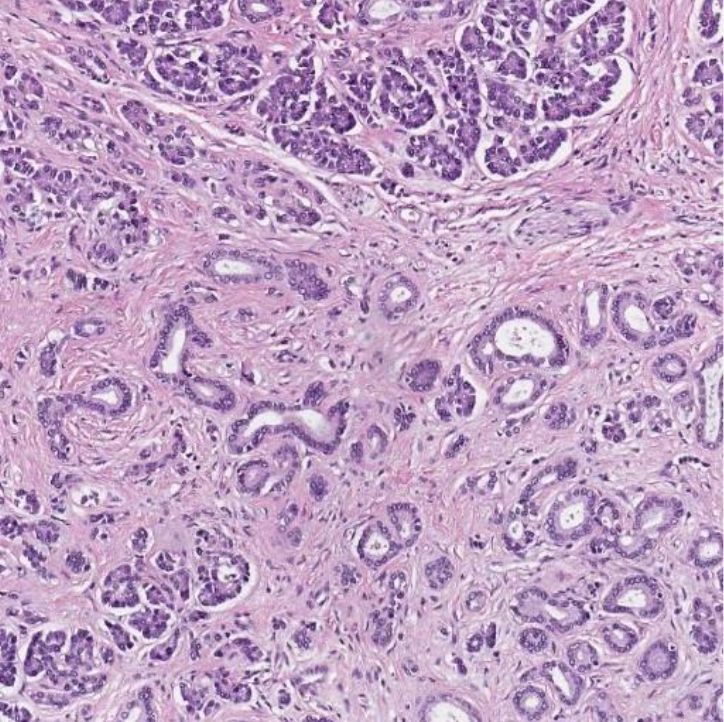
\includegraphics[width = \textwidth]{images/st_nn2}
                 \caption{}
                 \label{fig:st_nn2}
            \end{subfigure}
            \quad
            \begin{subfigure}[t]{0.3\textwidth}
                 \centering
                 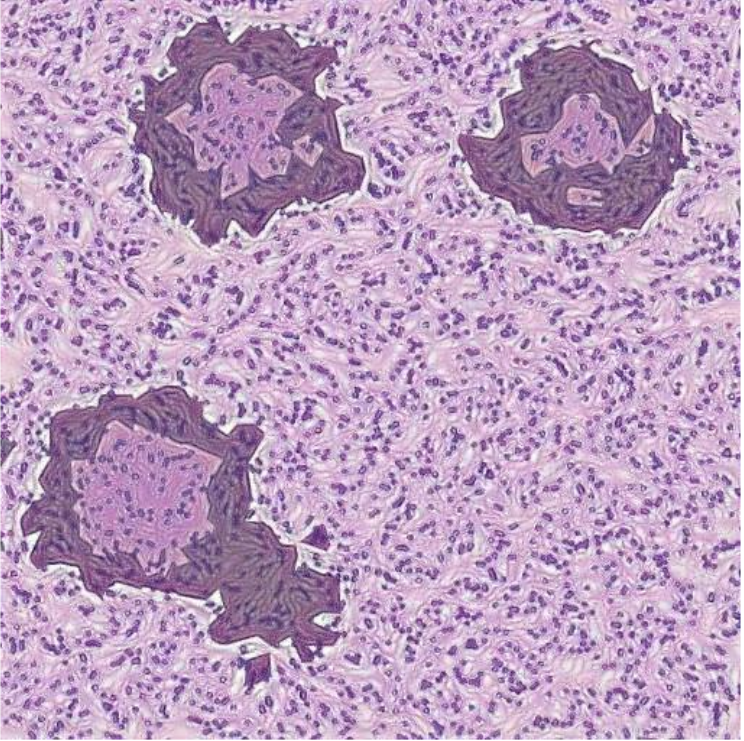
\includegraphics[width = \textwidth]{images/st_nn3}
                 \caption{}
                 \label{fig:st_nn3}
            \end{subfigure}
            \caption{Application of the style-transfer NN on a section of the pancreatic tissue model: \ref{fig:st_nn1} the content image, \ref{fig:st_nn2} the style image, \ref{fig:st_nn3} the hybrid resulting image.}
            \label{fig:panc_stnn}
        \end{figure}

        In Figures \ref{fig:panc_stnn}, and \ref{fig:derm_stnn} are reported the best results among all the different tests made on the sections. I made different tries on the same image with different processing before the manipulation with the STNN, to see the impact of the different adjustment on the resulting styled image. It tourned out that the presence of nuclei is essential to give an homogeneous texture to image and avoid unrealistic artifacts. On yhe other hand, the choice of the color palette has a way lighter effet than what one would think: the model yields almost the same result with a grey-levels image or with any other palette.

        It interesting to notice the timing cost of this style transfer operation. While all the other manipulation described in this chapter requires a very short time (seconds) to be applied, and are in practice \textit{instantaneous}, the trasfer of style is a way more robust operation, which implies the finalization of the tarining of a pre-trained neural network. On a computer with the technical specification described in section \ref{ssec:my_machine} this operation instead took minutes, which is a time two full orders of magnitude grater.

        \begin{figure}
            \centering
            \begin{subfigure}[t]{0.3\textwidth}
                 \centering
                 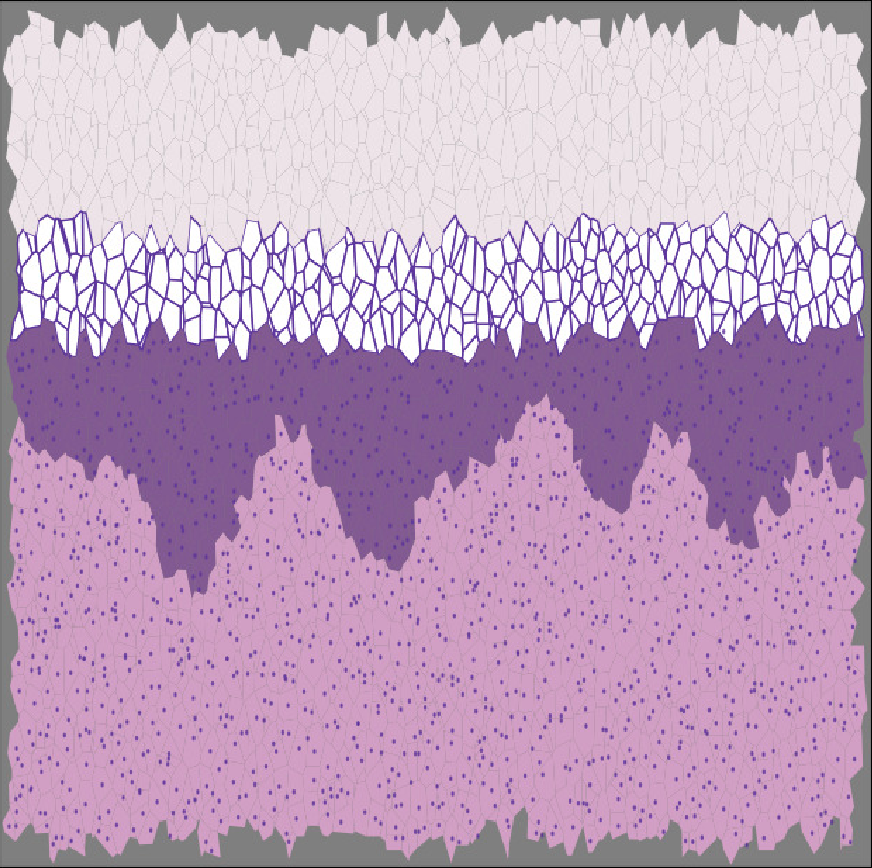
\includegraphics[width = \textwidth]{images/st_nn4}
                 \caption{}
                 \label{fig:st_nn4}
            \end{subfigure}
            \quad
            \begin{subfigure}[t]{0.3\textwidth}
                 \centering
                 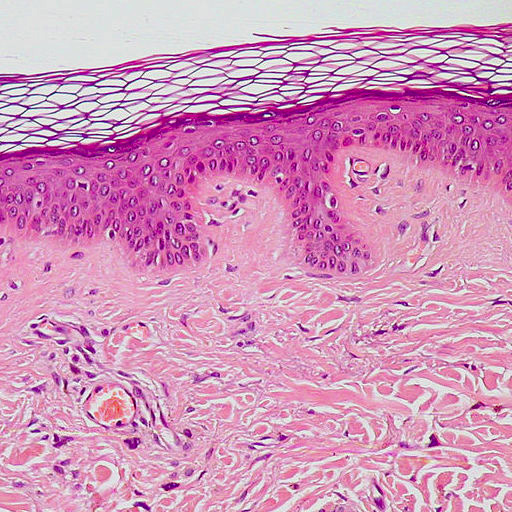
\includegraphics[width = \textwidth]{images/st_nn5}
                 \caption{}
                 \label{fig:st_nn5}
            \end{subfigure}
            \quad
            \begin{subfigure}[t]{0.3\textwidth}
                 \centering
                 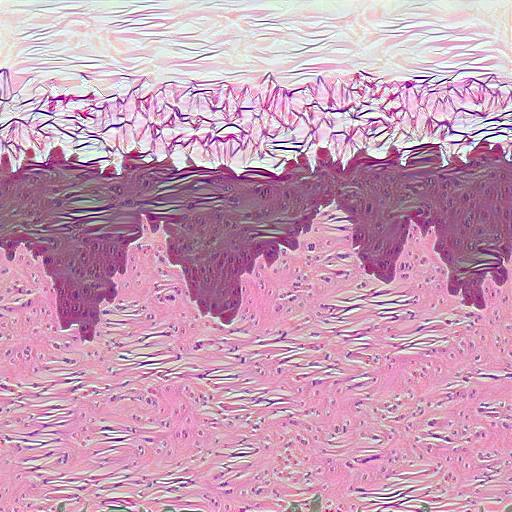
\includegraphics[width = \textwidth]{images/st_nn6}
                 \caption{}
                 \label{fig:st_nn6}
            \end{subfigure}
            \caption{Application of the style-transfer NN on a section of the dermal tissue model: \ref{fig:st_nn4} the content image, \ref{fig:st_nn5} the style image, \ref{fig:st_nn6} the hybrid resulting image.}
            \label{fig:derm_stnn}
        \end{figure}

        \hl{BEGIN COMMENT ON THE RESULTS}\\
        It should be noted that the presented results are obtained from the application of a pre-trained model. The development of a speciliazed model for histological texture transfer could\\
        \hl{END COMMENT ON THE RESULTS}

    \end{description}

One single complete application of the process consists then in the generation of a tissue model, in the sectioning along a random section plane and in the processing of the image, in order to produce the pair of ground-truth image and the synthetic histological image. The target is to apply over and over this process to collect the necessary amount of images and constitute an entire dataset. An important feature to have for the process in thus a complete automatization, in order to scale up the generation of images, possibly even in parallel computation.
For this purpose I created a pipeline workflow interface for the image generation, with an automatized harmonization of every piece of the process. The generation now requires just to fill a configuration file in which write all the spcific characteristics of the images: as the type of structrure, its features, the desired processing on the images, and eventually the random seeds for a supervised generation. In Figure \ref{fig:dataset} is reported a small scale example of dataset produced with multiple automatized applications of the generation tool on a ramificated structure inspired to a pancreatic tissue model. It is clear the correspondence between segmentation mask and synthetic histological images, and the diversification given by the supervised randomness on the generation.

The actual tool used for the set up of a working pipeline was the \texttt{Snakemake} \cite{10.1093/bioinformatics/bts480} workflow managment system, which is a python-based tool to create reproducible and scalable data analyses.

% ALTERNATIVE METHODS??? -> due articoli inviati ad Enrico
    \begin{figure}
        \centering
        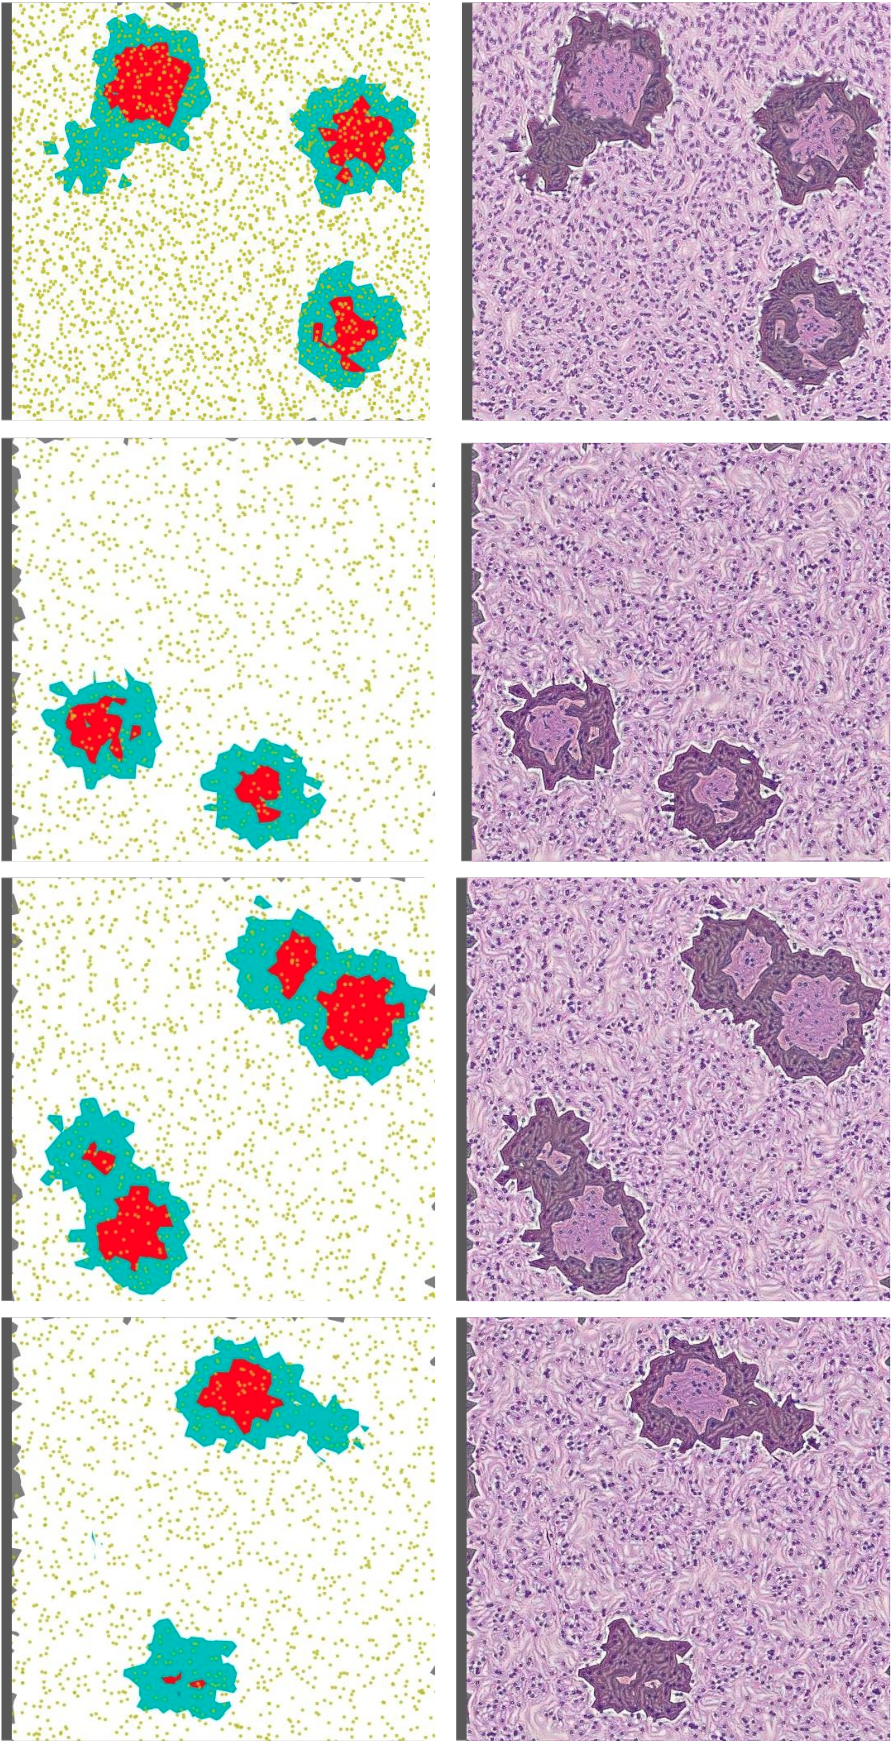
\includegraphics[height=20cm,keepaspectratio]{images/dataset}
        \caption{Small scale example of dataset produced with multiple automatized applications of the generation tool on a ramificated structure inspired to a pancreatic tissue model.}
        \label{fig:dataset}
    \end{figure}

\subsection{Alternative Works on Sythetic Histological Images Generation}
\hl{Alernative works.}
3 papers on the mail
